%% It is just an empty TeX file.
%% Write your code here.

\label{fs-drifting}

Most of the computational pipelines require state carrying between consecutive data items. For example, moving average calculation needs partial sums to be stored. The state management in distributed systems is a complicated topic that requires delicate treatment.

Some systems forces that all state management is put in business-logic: making state persistent, replication, ensuring state consistency, etc. Others shifts some difficulties to the system's concern, e.g., Flink provides a state API that guarantees consistency in case of failures \cite{Carbone:2017:SMA:3137765.3137777}. While it eases the heavy destiny of users, the core problem remains.

We propose a technique to simplify the development of stateful pipelines by eliminating the operation's state while remaining able to implement common transformations. We call this approach {\it drifting state}. The core idea is to make a state a part of the heterogeneous data flow. In order to do state updates, the drifting state is grouped with new elements, combined, and the new state is emitted. The limited number of such combines can be implemented with DAG by repetition of grouping and map operations. As stream processing is aimed to infinite sequences, there is a need for a cycle in the computational pipeline. The exact structure of such cycle is described in the following subsection with an example of typical stateful transformation, MapReduce.

The complex graph with multiple stateful operators can be constructed using a cycle for each stateful component. It is important to say that such tangled structures may not be exposed to the end-user and can be hidden by some high-level API.

\subsection{MapReduce transformation}
Map stage of MapReduce can be formulated directly in terms of our map operation. The algorithm~\ref{reduce} shows a generic reduce stage. The {\it accumulator} is an explicit state that should be kept between subsequent iterations.

\begin{algorithm}
\caption{Generic reduce stage}
\label{reduce}
\begin{algorithmic}
  \Function{reduce}{$key$, $values$}
    \State $accumulator$ \Comment{reduce's state}
    \ForAll{$v \in values$} 
      \State \Call{combine}{$v$, $accumulator$}
    \EndFor
    \State \Return \Call{map}{$accumulator$}
  \EndFunction
\end{algorithmic}
\end{algorithm}

To implement reduce stage we apply the drifting state idea and make the accumulator value a part of the stream. Figure~\ref{mapreduce-graph-figure} shows a generic graph for MapReduce transformation. Map and reduce stages are highlighted with a dashed line. 

\begin{figure}[htb]
  \centering
  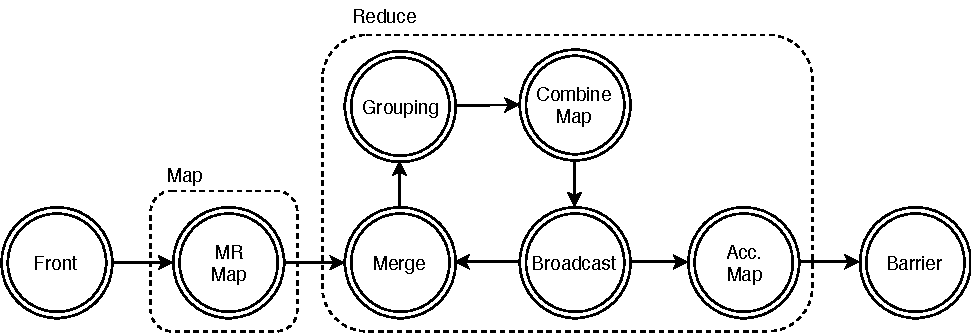
\includegraphics[scale=0.5]{pics/mapreduce}
  \caption{Logical graph for MapReduce transformations}
  \label {mapreduce-graph-figure}
\end{figure}

There are four types of data items in this stream: {\it input}, {\it mapped}, {\it accumulator}, {\it and reduced} items. Mapped, accumulator and reduced items have the key-value structure of a payload. The operations of the stream have the following purposes:

\begin{itemize}
  \item The first map operation accepts input items, and outputs mapped items according to map stage of MapReduce model
  \item The window of grouping is set to 2. It is used to group current accumulator with next data item to combine them further. The hash function is designed to return distinct values for payloads with distinct keys
  \item The second map implements the actual combining. It accepts inputs that have a form of: \textit{(mapped item)} or \textit{(accumulator item, mapped item)}. The first kind is transformed into some initial value. The second one is combined into the new accumulator item as specified by reduce stage of MapReduce. The tuples with structure \textit{(mapped item, accumulator item)} are filtered out
  \item The third map is the accumulator map. It accepts accumulator items and applies the final map transformation to them
\end{itemize}

The fundamental idea is that ordering assumptions about data items guarantees that each accumulator item always arrives at the grouping right after previous mapped item and before a new one. Hence, each mapped item that has not been combined yet would be grouped with the right accumulator item. Additionally, when combine map accepts tuple {\it (mapped item, accumulator item)}, then it means that mapped item was generated before accumulator item, and therefore, it had been already combined. The cycle gives the ability for new accumulator items to get back in the grouping operation. The accumulator map transforms the accumulator item into the final reduced item right before sink. Thereby, the stream reacts to each input item by generating new reduced item, which contains the actual value of the reduce stage.

\subsection{Example: word count}

We illustrate the MapReduce algorithm with an example of word counting. Map stage of this algorithm transforms each input word into key-value pair where the word is a key, and the value is 1. Reduce stage sums all values into the final result for the specific key. In this case, the accumulator map is omitted, because the accumulator is the actual result of the reduce stage.

The example of input/output items, which are generated/ transformed by the part of the logical graph, is shown in Figure~\ref {word-count-figure}. According to our graph for MapReduce transformations, the item {\it m[dog, 1]} represents mapped item with key "dog" and value 1. The item {\it a[dog, 1]} describes accumulator item with key "dog" and value 1. Figure shows how the model reacts on two consequent input items containing word "dog". The meta-information of items is omitted for simplification. More precisely, there are four stages separated by dotted lines:

\begin{enumerate}
    \item New mapped item with key "dog" arrives at grouping with an empty state. Grouping outputs tuple with this single item. Combine map transforms it into the first accumulator item for key "dog" and value 1.
    \item The accumulator item arrives at grouping after it went through the cycle. It is grouped in the tuple with the mapped item that has been already in the state with key "dog". However, combine map drops this tuple, because of the order of items.
    \item New mapped item with key "dog" arrives at grouping. It is inserted right after the accumulator in the bucket for key "dog". The grouping operation outputs tuple containing the accumulator item and new mapped item. Map operation combines reduced and mapped items into new reduced items with key "dog" and value 2.
    \item New accumulator item arrives at grouping through the cycle, but new generated tuple is not accepted by combine map, as well as in step 2.
\end{enumerate}

\begin{figure}[htb]
  \centering
  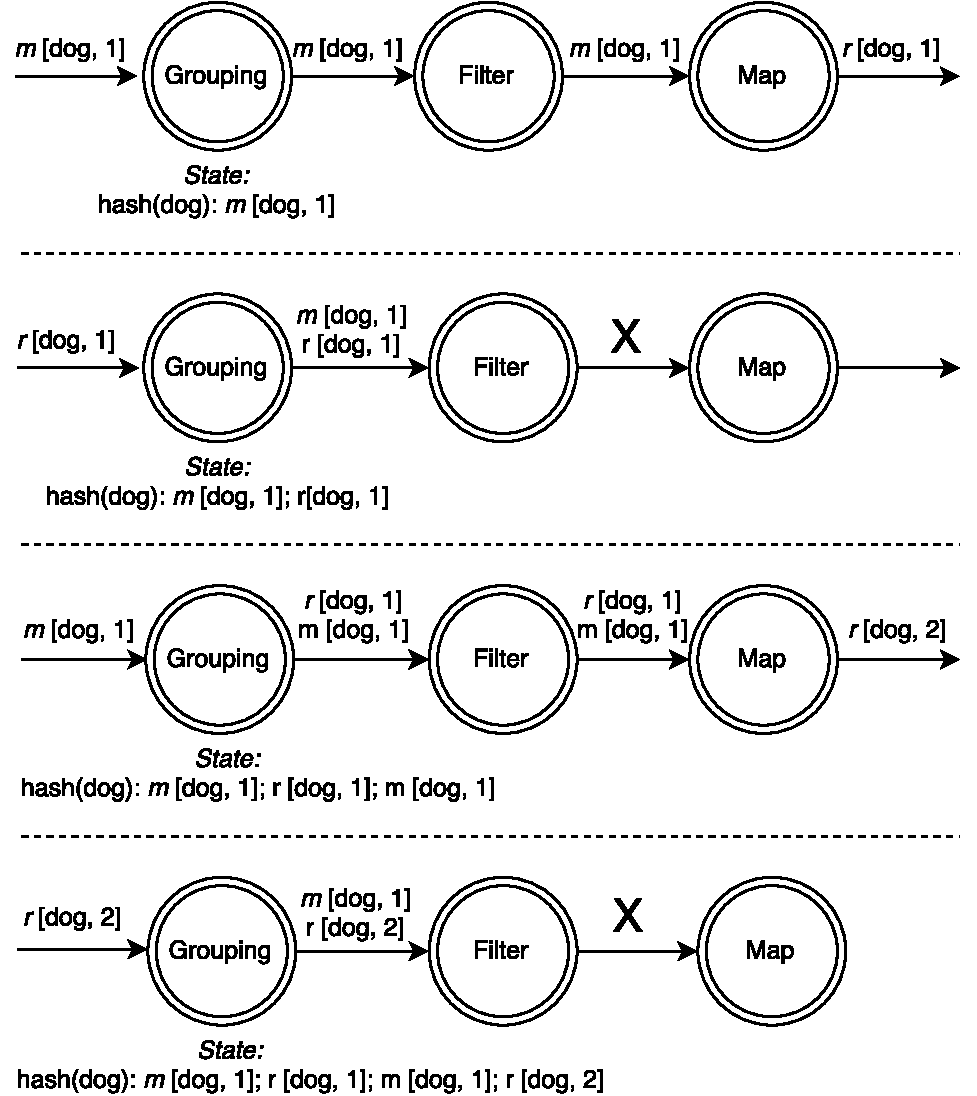
\includegraphics[scale=0.5]{pics/wordcount}
  \caption{The example of input/output items, which are generated/ transformed by the part of the logical graph for word counting}
  \label {word-count-figure}
\end{figure}
